\subsection{Effektivitet}

\centerline{\textbf{Hur viktigt är effektivitet för 
din användarupplevelse}}
\begin{figure}[H]
  \centering
  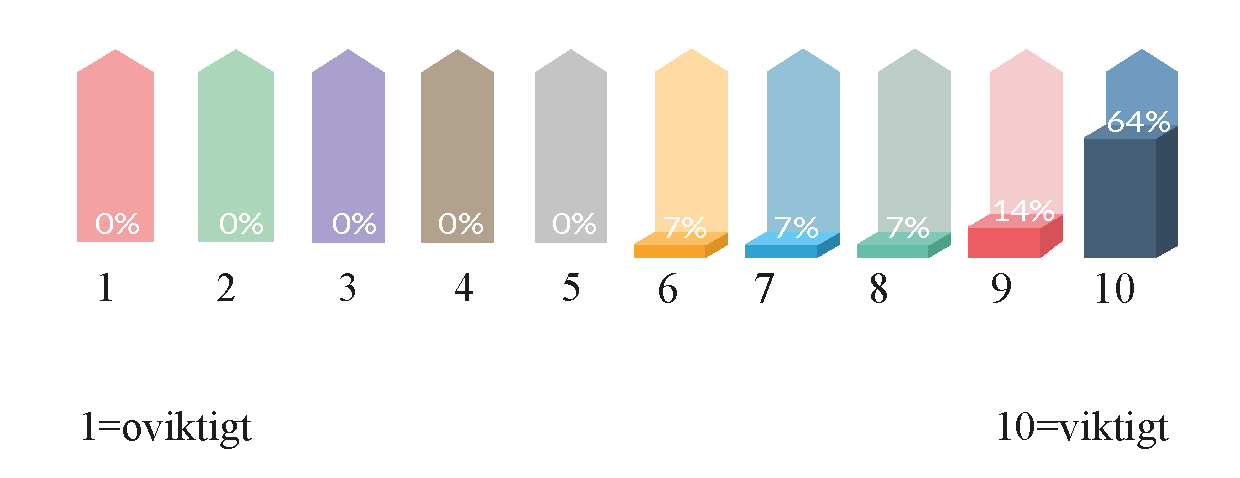
\includegraphics[scale=0.7]{Rityta_9.pdf}
\centering
\captionsetup{justification=centering,margin=2cm}
\caption{Resultat i procentuell skala på respondenternas svar}
\end{figure} 

Medelvärdet av ovan figur är 9.2. Siffran representerar ett medelvärde av stapeldiagrammet som visar hur viktigt det var för användarupplevelsen enligt kategoriseringen framtagen av Laugwitz et al. \cite{Laugwitz2008ConstructionQuestionnaire}.

%\[
 % m= 9.2
  %m = \frac{6+ 7+ 8 + 18 + 90}{14} = 9.2
  %\]

%Med en standardavvikelse på
%\[
 % \sigma = \sqrt{V} = \sqrt{ \frac{(6-1)^{2} + (7-1)^{2} + (8-1)^{2} + (9-2)^{2} + (10-9)^{2}} {5} } =  \sqrt{32} = 5.7
  %  \]

\begin{figure}[H]
  \centering
  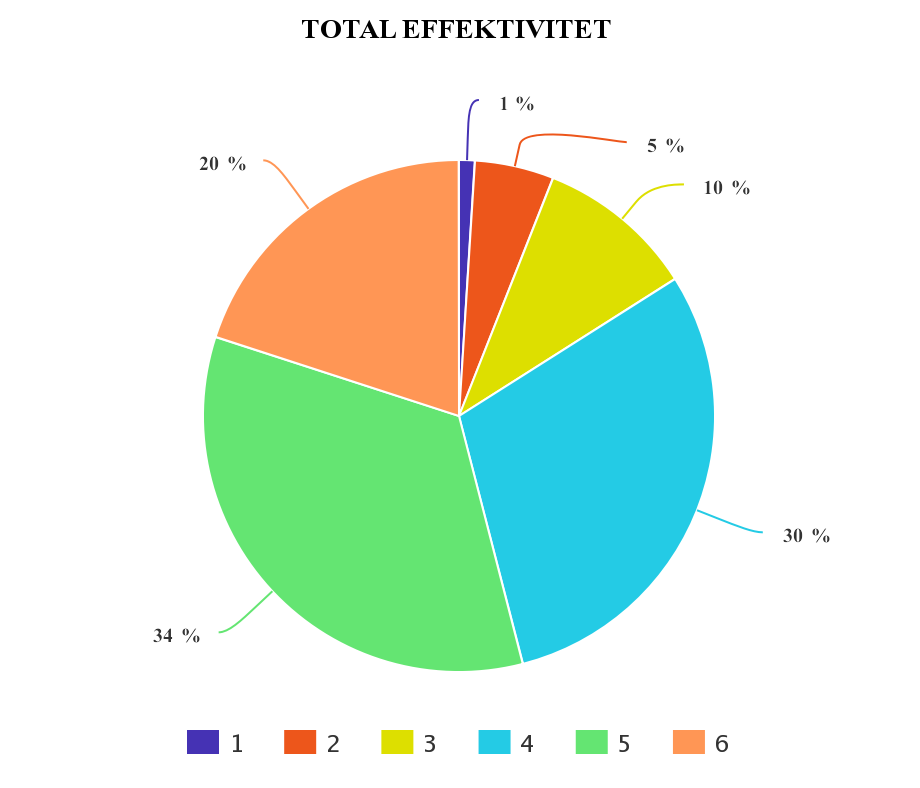
\includegraphics[scale=0.4]{meta-chart-3.png}
  \captionsetup{justification=centering,margin=2cm}
 \caption{Resultat av total effektivitet}
\end{figure} 
Figuren visar det slutgiltiga resultatet från både enkätundersökningen samt fokusgrupperna. Figuren visar sambandet mellan hur viktigt effektivitet är för användarupplevelsen i en applikation kontra hur effektiv prototypen känts. Den första rutan visar på hur viktigt det är för användaren att en applikation är effektiv, enligt personerna som medverkade i fokusgrupperna. Denna siffran beräknades med hjälp av snitt och varians och presenteras nedan. Diagrammen visar på hur effektiv prototypen kändes, enligt användarna som svarade på enkätundersökningen. 

\textbf{Citat från fokusgrupperna}
\begin{quotation}
\em Absolut är det viktigt att allting fungerar smidigt och att man kommer till nästa steg snabbt.
\end{quotation}

\begin{quotation}
\em  Effektivitet i alla former av digitala produkter är en självklarhet för mig. Ifall det buggar massvis hade jag inte orkat vara inne på applikationen och tagit det som att den inte är välgjort.
\end{quotation}

\begin{quotation}
\em Den tekniska delen är något man inte tänker på så mycket, man tar för givet att det ska fungera.
\end{quotation}
